\section{Impressum}
Das Impressum beinhaltet die drei Schüler, die die Diplomarbeit ausarbeitet haben, und deren Betreuer.
\subsection{Projektteam}
Das Projektteam besteht aus folgenden Schülern:

\bigskip

\begin{table}[H]
  \centering
  \begin{tabular}{lp{0.4\textwidth}c}
    \multicolumn{3}{c}{\textbf{Projektteam}}                                                                                                                                                                                                                                                                                                                                      \\
    \toprule
    Paul Hartmann  & Paul übernahm die Projektleitung und war für die Kommunikation mit dem Partnerunternehmen zuständig. Er recherchierte zu Varianten zur Lagerung von Fahrrädern und führte die Nutzwertanalyse und Umfrage aus. Paul entwickelte die Mobile-App.          & \begin{minipage}{.3\textwidth}\centering
\includegraphics{images/paulhartmann.jpg} \end{minipage}  \\
    \midrule
    Joshua Lung    & Joshua recherchierte zu Varianten zur Lagerung von Fahrrädern, führte die Nutzwertanalyse aus, erstellte Fragen der Umfrage und konzeptionierte das Rondell-Modell. Er baute den Prototyp des Turmes und übernahm die Softwareentwicklung der Steuerung. & \begin{minipage}{.3\textwidth}\centering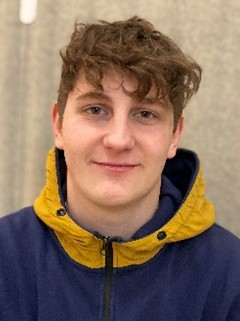
\includegraphics{images/joshualung.jpg} \end{minipage}    \\
    \midrule
    Lukas Madlener & Lukas erstellte Skizzen für verschiedene automatisierte Arten zur Lagerung von Fahrräadern und konzeptionierte das Hochregallager. Er testete NFCTechnologien mit einer Mobile-App.                                                                      & \begin{minipage}{.3\textwidth}\centering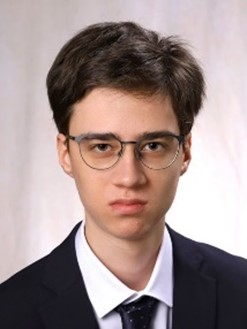
\includegraphics{images/lukasmadlener.jpg} \end{minipage} \\
    \bottomrule
  \end{tabular}
  \caption{Projektteam}
  \label{tab:projektteam}
\end{table}

\subsection{Projektbetreuer der Schule}
\begin{table}[H]
  \centering
  \begin{tabular}{lp{0.4\textwidth}c}                         \\
    \multicolumn{3}{c}{\textbf{Projektbetreuer}} \\
    \toprule
    \makecell[l]{Prof. MMag.                     \\Hämmerle Günter} & Günter Hämmerle initiierte das Projekt mit dem Partnerunternehmen LTW Intralogistics und war bei allen Besprechungen mit dem Partnerunternehmen dabei. Er unterstützte das Team in allen Projektphasen, besonders bei der Analyse der Kosten und der Dokumentation der Diplomarbeit. & \begin{minipage}{.3\textwidth}\centering
\includegraphics{images/günterhämmerle.jpg} \end{minipage} \\
    \midrule
    \makecell[l]{Prof. Mag.                      \\Riedmann Andreas} & Andreas Riedmann unterstützte das Team bei der Softwareentwicklung des Prototypen und bei der Dokumentation der Diplomarbeit. & \begin{minipage}{.3\textwidth}\centering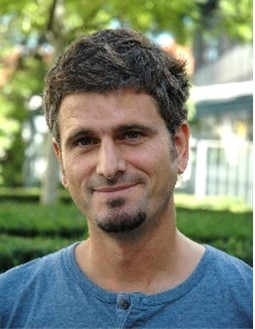
\includegraphics{images/andreasriedmann.jpg} \end{minipage} \\
    \bottomrule
  \end{tabular}
  \caption{Projektbetreuer}
  \label{tab:projektbetreuer}
\end{table}

\subsection{Projektbetreuer vom Partnerunternehmen}
Johannes Schwartze war der Betreuer der Diplomarbeit vonseiten des Partnerunternehmens LTW Intralogistics. Er war der Ansprechpartner bei Fragen und gab neue Aufgabestellungen und Feedback. Beim Partnerunternehmen gab es mehrere Besprechungen, wo die Fortschritte präsentiert und diskutiert wurden.  \\